\section{Background: Broadside and Basejump}

Action and the Basejump platform were inspired by the \href{https://opensea.io/collection/broadside/activity}{Broadside} community. Broadside began life in 2022 as an NFT project. The community that gathered around it quickly became one of the most active communities in the open metaverse. Watching how the Broadsiders came together to use blockchain connected assets across games, worlds and social platforms inspired the idea for hyperobjects and the Action substrate. As a result, the team behind Broadside created two key components to bootstrap development of the Action ecosystem:

\nopagebreak[4]
\begin{itemize}
\item The first collection of hyperobjects: Broadside OGs
\item The first application built on Action: Basejump
\end{itemize}


\begin{figure}
  \centering
  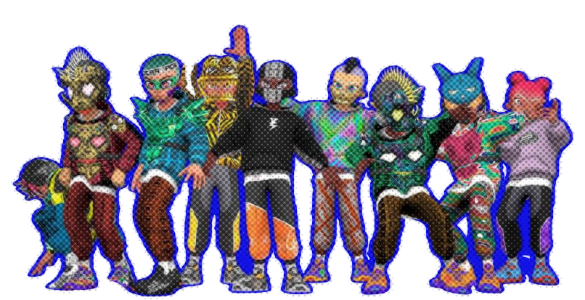
\includegraphics[width=\columnwidth]{images/image9.png}
  \caption{Broadside OG Action Figures, built using the VRM file format \cite{VRM2024}}
  \label{fig:broadside_og}
  \end{figure}

\subsection{Broadside OGs}

The Broadside OG collection has been converted to interoperable VRM \cite{VRM2024} avatars known as 'Action Figures' (Figure \ref{fig:broadside_og}) - concept cars designed to demonstrate the possibilities of hyperobjects that can:

\begin{itemize}
\item Unlock and use new Action Items, including weapons, clothing and armor
\item Earn the highest multipliers on both Basejump XP and ACTION
\item Feature AI text to speech functionality on Basejump in 300+ voices and 30 languages
\item Are compatible with thousands of experiences, worlds, games and platforms
\item Will continuously be upgraded with experimental new features
\end{itemize}


\subsection{Basejump}  

Basejump is a no-code surface that makes it easy to make, discover and monetize games and assets compatible with every platform, powered by the Action substrate.

\begin{itemize}
\item Most game creation platforms are toolsets. Basejump is a consumer focused, avatar-centric surface (Figure \ref{fig:basejump_platform}) with a deeply rewarding core game loop
\item Basejump's first core game (Figure \ref{fig:basejump_battle}) launches Spring 2025 on the web and natively in Discord
\item Basejump will be dropping new hyperobject collections with games, platforms, brands and artists designed to showcase hyperobject capabilities. Collaborations with Nifty Island and the Korus platform have driven early engagement, and a project with the hit Netflix show Black Mirror has been \href{https://x.com/blackmirror_xp/status/1786108170311541244}{announced}, in partnership with game studio Pixelynx
\item The Basejump creator hub is live now: \href{https://basejump.xyz/}{\texttt{basejump.xyz}}
\end{itemize}

\begin{figure}[t]
\centering
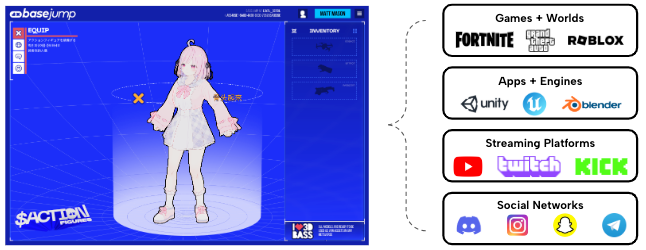
\includegraphics[width=\columnwidth]{images/image10.png}
\caption{Basejump makes it easy to make, discover and monetize games and assets compatible with every platform}
\label{fig:basejump_platform}
\end{figure}

\begin{figure}[t]
\centering
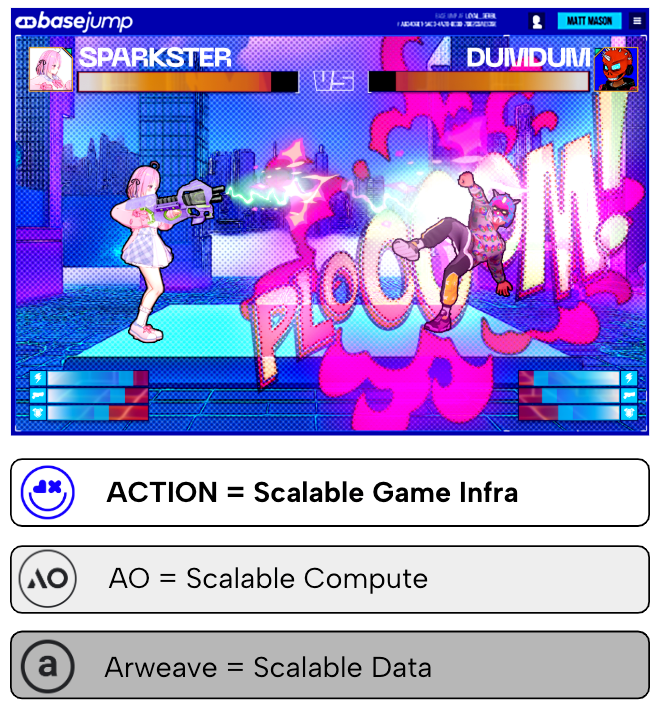
\includegraphics[width=\columnwidth]{images/image11.png}
\caption{Basejump runs as a PVP Battle game for hyperobjects in Discord and on the web, powered by Action, AO and Arweave.}
\label{fig:basejump_battle}
\end{figure}
